\documentclass{beamer}

\usepackage[english,russian]{babel}
\hypersetup{unicode=true}
\graphicspath{ {images/} }

\title{Реализация редизайна главного экрана приложения «Яндекс — с Алисой»}
\author{Глушень Павел Владимирович, группа 244}
\date{}

\begin{document}

\begin{frame}
\titlepage
\begin{flushright}
    Научный руководитель: \\
    к.т.н., доц. Ю.В. Литвинов
    \end{flushright}    
\end{frame}

\begin{frame}{Введение}
    \begin{figure}[h]
        \includegraphics[width=\textwidth]{2-bender-compare}
        \caption{Слева Бендер до редизайна, справа — после}
    \end{figure}
\end{frame}

\begin{frame}{Постановка задачи}
    Целью работы является реализация нового Бендера.
    
    Требуется:
    \begin{itemize}
        \item Разработать архитектуру для нового Бендера
        \begin{itemize}
            \item Декомпозировать задачу
            \item Описать базовый макет
            \item Описать архитектуру компонента
        \end{itemize}
        \item Реализовать новый Бендер, решив каждую подзадачу,
        появившуюся в результате декомпозиции
    \end{itemize}
\end{frame}

\begin{frame}{Декомпозиция задачи}
    Нужно реализовать:
    \begin{itemize}
        \item Кнопку меню
        \item Строку статуса
        \item Счетчик количества открытых браузерных вкладок
        \item Логотип, который может заменяться на произвольную картинку
        \item Омнибокс с кнопкой камеры
        \item Информеры погоды, дорожного трафика, почты и чатов
        \item Вкладки сервисов
    \end{itemize}

    После нужно реализовать анимацию схлопывания.
\end{frame}

\begin{frame}{Базовый макет}
    \begin{figure}[h]
        \center{\includegraphics[scale=0.25]{3-2-vertical}}
        \caption{Визуализация корневого элемента верстки}
    \end{figure}
\end{frame}

\begin{frame}{Архитектура компонента}
    \begin{figure}[h]
        \center{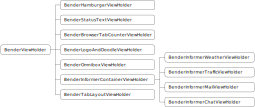
\includegraphics[width=\textwidth]{3-2-hierarchy}}
        \caption{Иерархия классов, реализующих функциональность Бендера}
    \end{figure}
\end{frame}

\begin{frame}{Результаты}
    В результате работы:
    \begin{itemize}
        \item Разработана архитектура компонента
        \begin{itemize}
            \item Декомпозирован проект
            \item Разработан базовый макет
            \item Разработана базовая архитектура;
        \end{itemize}
        \item Решены возникшие подзадачи, то есть реализованы:
        \begin{itemize}
            \item Кнопка меню
            \item Строка статуса
            \item Счетчик количества браузерных вкладок
            \item Логотип
            \item Омнибокс с кнопкой камеры
            \item Информеры погоды, дорожного трафика, почты и чатов
            \item Вкладки сервисов
            \item Анимация схлопывания
        \end{itemize}
    \end{itemize}

    Результат работы стал частью приложения \mbox{«Яндекс — с Алисой»}.
\end{frame}

\end{document}
